\documentclass{article}\usepackage[]{graphicx}\usepackage[]{xcolor}
% maxwidth is the original width if it is less than linewidth
% otherwise use linewidth (to make sure the graphics do not exceed the margin)
\makeatletter
\def\maxwidth{ %
  \ifdim\Gin@nat@width>\linewidth
    \linewidth
  \else
    \Gin@nat@width
  \fi
}
\makeatother

\definecolor{fgcolor}{rgb}{0.345, 0.345, 0.345}
\newcommand{\hlnum}[1]{\textcolor[rgb]{0.686,0.059,0.569}{#1}}%
\newcommand{\hlsng}[1]{\textcolor[rgb]{0.192,0.494,0.8}{#1}}%
\newcommand{\hlcom}[1]{\textcolor[rgb]{0.678,0.584,0.686}{\textit{#1}}}%
\newcommand{\hlopt}[1]{\textcolor[rgb]{0,0,0}{#1}}%
\newcommand{\hldef}[1]{\textcolor[rgb]{0.345,0.345,0.345}{#1}}%
\newcommand{\hlkwa}[1]{\textcolor[rgb]{0.161,0.373,0.58}{\textbf{#1}}}%
\newcommand{\hlkwb}[1]{\textcolor[rgb]{0.69,0.353,0.396}{#1}}%
\newcommand{\hlkwc}[1]{\textcolor[rgb]{0.333,0.667,0.333}{#1}}%
\newcommand{\hlkwd}[1]{\textcolor[rgb]{0.737,0.353,0.396}{\textbf{#1}}}%
\let\hlipl\hlkwb

\usepackage{framed}
\makeatletter
\newenvironment{kframe}{%
 \def\at@end@of@kframe{}%
 \ifinner\ifhmode%
  \def\at@end@of@kframe{\end{minipage}}%
  \begin{minipage}{\columnwidth}%
 \fi\fi%
 \def\FrameCommand##1{\hskip\@totalleftmargin \hskip-\fboxsep
 \colorbox{shadecolor}{##1}\hskip-\fboxsep
     % There is no \\@totalrightmargin, so:
     \hskip-\linewidth \hskip-\@totalleftmargin \hskip\columnwidth}%
 \MakeFramed {\advance\hsize-\width
   \@totalleftmargin\z@ \linewidth\hsize
   \@setminipage}}%
 {\par\unskip\endMakeFramed%
 \at@end@of@kframe}
\makeatother

\definecolor{shadecolor}{rgb}{.97, .97, .97}
\definecolor{messagecolor}{rgb}{0, 0, 0}
\definecolor{warningcolor}{rgb}{1, 0, 1}
\definecolor{errorcolor}{rgb}{1, 0, 0}
\newenvironment{knitrout}{}{} % an empty environment to be redefined in TeX

\usepackage{alltt}
\usepackage{amsmath} %This allows me to use the align functionality.
                     %If you find yourself trying to replicate
                     %something you found online, ensure you're
                     %loading the necessary packages!
\usepackage{amsfonts}%Math font
\usepackage{graphicx}%For including graphics
\usepackage{hyperref}%For Hyperlinks
\usepackage[shortlabels]{enumitem}% For enumerated lists with labels specified
                                  % We had to run tlmgr_install("enumitem") in R
\hypersetup{colorlinks = true,citecolor=black} %set citations to have black (not green) color
\usepackage{natbib}        %For the bibliography
\setlength{\bibsep}{0pt plus 0.3ex}
\bibliographystyle{apalike}%For the bibliography
\usepackage[margin=0.50in]{geometry}
\usepackage{float}
\usepackage{multicol}
%fix for figures
\usepackage{caption}
\newenvironment{Figure}
  {\par\medskip\noindent\minipage{\linewidth}}
  {\endminipage\par\medskip}
\IfFileExists{upquote.sty}{\usepackage{upquote}}{}
\begin{document}

\vspace{-1in}
\title{Lab 08 -- MATH 240 -- Computational Statistics}

\author{
  Brendan Mariano \\
  Colgate University  \\
  Mathematics  \\
  {\tt bmariano@colgate.edu}
}

\date{}

\maketitle

\begin{multicols}{2}
\begin{abstract}
This lab provides a template for understanding how 

This document provides a basic template for the 2-page labs we will complete each week. Here, briefly summarize what you did and why it might be helpful. Provide all the top-line conclusions, but avoid providing \emph{all} the details. Results should be limited to ``we show X, Y, and Z."
\end{abstract}

\noindent \textbf{Keywords:} What topics does the lab cover concerning class? List 3-4 key terms here, separated by semicolons.

\section{Introduction}
In this lab, we sought to determine whether the 
Provide an overarching summary of what you're talking about. In this section, you introduce the idea to the reader, and your goal is to pull them in. What's the mystery you aim to solve?

You want to provide enough background to understand the context of the work. Specifically, what is the question you are addressing? If it applies, describe what information currently exists about this problem, including citations, and explain how the question you're answering complements this work.

Provide a roadmap of the structure of the paper. 

\subsection{Intro Subsection}
You might need/want to discuss the topics in subsections. Or, you may have multiple questions.

\section{Density Functions and Parameters}
  We began by producing the beta probability density function with four different parameters for alpha and beta: (2,5), (5,5), (5,2), and (.5,.5). Using the data and ggplot citep{ggplot2}, we produced individual graphs for each set of parameters which also had a normal distribution containing the same mean and variance. Additionally, we included a Gaussian distribution in the plot which has the same mean and variance as the Beta distribution. When alpha and beta were equal at (5,5), the beta distribution resembled a normal distribution. When we decreased alpha to two, however, the data became right skewed, and when we decreased beta to two, the distribution became left skewed. Lastly, when we decreased both the alpha and beta to less than one, the distribution was symmetrical but had a greater density on the tails. 
  
  
   \begin{figure}[H]
    \begin{center}
       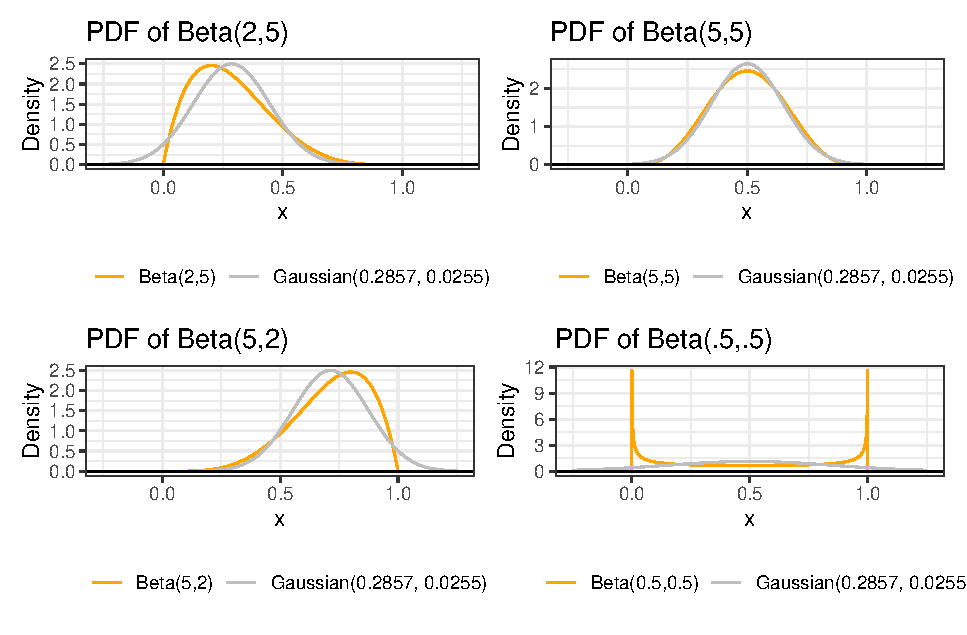
\includegraphics[scale=0.5]{densityf.pdf}
       \caption{}
     \label{densityf}
     \end{center}
   \end{figure}



We used data about the death rates worldwide in 2022. We cleaned the data using the tidyverse \citep{tidyverse} 
and made it usable for a beta distribution (having every value between 0 and 1 inclusive). 
Since our overall goal was to compare the MLE and MOM, we calculated the values for each estimation  
method using R. We also created a graph using ggplot \citep{ggplot2} comparing the population distribution in a histogram to the MLE and 
MOM which were different colored lines.
After working with the data from the worldwide death rates, we created 1000 samples of data using set seed 
so that we could calculate that alpha and beta values for each point estimation method. Using the 1,000 
values for MLE alpha, MLE, beta, MOM alpha and MOM beta, we were able to create graphs that compared the MLE 
to the MOM.
death rates in from almost every part of the world in 2022. This 
Describe the data you are working with, if applicable. Describe the specific process you will follow to answer the question at hand. This does not mean you should write something like this.
\begin{quote}
\textit{I did this and then I did that and then I did this other thing and then..., and then..., and then...}
\end{quote}
Instead, it should provide a clear and concise narrative that flows from the problem specification in the Introduction to how you will approach answering it. This is where I would expect to see some citations for \texttt{R} packages you will use to conduct the statistical analysis reported in the Results section.


\subsection{Methods Subsection}
Much like the Introduction, subsections can be helpful for the Methods section. For example, you might describe data collection and the statistical analyses of the collected data in different subsections. Or, you may have different questions that require distinct methods. 

\section{Properties}
There were four properties or moments, which we analyzed: mean, variance, skewness, and kurtosis. Moments are different indicators for a distribution. They can either be uncentered, indicating that they take they don't account for the mean, or centered which means that they account for the mean. The moments are advantageous because they allow us to calculate the values for a sample. The equations are as follows. 


\[
\mu_X = \mathbb{E}(X)
\]

\[
\sigma_X^2 = \mathrm{var}(X) = \mathbb{E} \left[ (X - \mu_X)^2 \right]
\]

\[
\mathrm{skew}(X) = \frac{\mathbb{E} \left[ (X - \mu_X)^3 \right]}{\left( \mathbb{E} \left[ (X - \mu_X)^2 \right] \right)^{3/2}}
\]

\[
\mathrm{kurt}(X) = \frac{\mathbb{E} \left[ (X - \mu_X)^4 \right]}{\left( \mathbb{E} \left[ (X - \mu_X)^2 \right] \right)^2} - 3
\]





When we created our plot comparing the actual death rates in 2022 to the MLE and MOM estimations, we found that they were all distributed very similarly. The MLE and MOM distributions were practically identical and the population histogram followed a very similar shape to the lines. 

For our four plots comparing the distribution of Alpha and Beta values for MLE and MOM over 1,000 samples, the MLE had a 
more defined peak for both the Alpha and Beta values. The alpha value peaked at roughly 8 and the beta value 
peaked at roughly 950. The distribution of MOM values also peaked at 8 for alpha and 950 for beta, however, the peak is 
less sharp which suggests more variance within the data.  

TALK ABOUT TABLE
ADD TABLE AND GRAPHS
Tie together the Introduction -- where you introduce the problem at hand -- and the methods --  what you propose to do to answer the question. Present your data, the results of your analyses, and how each reported aspect contributes to answering the question. This section should include table(s), statistic(s), and graphical displays. Make sure to put the results in a sensible order and that each result contributes a logical and developed solution. It should not just be a list. Avoid being repetitive. 

\subsection{Results Subsection}
Subsections can be helpful for the Results section, too. This can be particularly helpful if you have different questions to answer. 


\section{Example}

 You should objectively evaluate the evidence you found in the data. Do not embellish or wish-terpet (my made-up phase for making an interpretation you, or the researcher, wants to be true without the data \emph{actually} supporting it). Connect your findings to the existing information you provided in the Introduction.

Finally, provide some concluding remarks that tie together the entire paper. Think of the last part of the results as abstract-like. Tell the reader what they just consumed -- what's the takeaway message?

%%%%%%%%%%%%%%%%%%%%%%%%%%%%%%%%%%%%%%%%%%%%%%%%%%%%%%%%%%%%%%%%%%%%%%%%%%%%%%%%
% Bibliography
%%%%%%%%%%%%%%%%%%%%%%%%%%%%%%%%%%%%%%%%%%%%%%%%%%%%%%%%%%%%%%%%%%%%%%%%%%%%%%%%
\vspace{2em}

\noindent\textbf{Bibliography:} Note that when you add citations to your bib.bib file \emph{and}
you cite them in your document, the bibliography section will automatically populate here.

\begin{tiny}
\bibliography{bib}
\end{tiny}
\end{multicols}

%%%%%%%%%%%%%%%%%%%%%%%%%%%%%%%%%%%%%%%%%%%%%%%%%%%%%%%%%%%%%%%%%%%%%%%%%%%%%%%%
% Appendix
%%%%%%%%%%%%%%%%%%%%%%%%%%%%%%%%%%%%%%%%%%%%%%%%%%%%%%%%%%%%%%%%%%%%%%%%%%%%%%%%
\newpage
\onecolumn
\section{Appendix}
\begin{table}[ht]
\centering
\begin{tabular}{rlrrr}
  \hline
 & Element & Bias & Precision & MSE \\ 
  \hline
1 & Alpha (MLE) & 0.07 & 2.13 & 0.48 \\ 
  2 & Beta (MLE) & 9.11 & 0.00 & 7132.70 \\ 
  3 & Alpha (MOM) & 0.08 & 1.83 & 0.55 \\ 
  4 & Beta (MLE) & 10.29 & 0.00 & 8288.46 \\ 
   \hline
\end{tabular}
\end{table}
If you have anything extra, you can add it here in the appendix. This can include images or tables that don't work well in the two-page setup, code snippets you might want to share, etc.

\end{document}
